% !TEX encoding = UTF-8
%Koma article
\documentclass[fontsize=12pt,paper=letter,twoside]{scrartcl}
\usepackage{float}
\usepackage{listings}
\usepackage{makecell}

%Standard Pre-amble
\usepackage[top=4cm,bottom=4cm,left=3cm,right=3cm,asymmetric]{geometry}
%\geometry{landscape}                % Activate for for rotated page geometry
%\usepackage[parfill]{parskip}    % Begin paragraphs with an empty line rather than an indent
\usepackage[table,xcdraw]{xcolor}
\usepackage{graphicx}

\usepackage{amsmath}
\usepackage{amssymb}
\usepackage{epstopdf}
\DeclareGraphicsRule{.tif}{png}{.png}{`convert #1 `dirname #1`/`basename #1 .tif`.png}
% Listings needs package courier
\usepackage{listings} % Needs 
\usepackage{courier}

\usepackage[framemethod=TikZ]{mdframed}
\usepackage{url}

\usepackage{sty/bsymb} %% Event-B symbols
\usepackage{sty/eventB} %% REQ and ENV
\usepackage{sty/calculation}

%Maths
\usepackage{amssymb,amsmath}
\def\Fl{\mathbb{F}}
\def\Rl{\mathbb{R}}
\def\Nl{\mathbb{N}}
\def\Bl{\mathbb{B}}
\def\St{\mathbb{S}}
\newcommand{\ovr}{\upharpoonright}
\newcommand{\var}[1]{\textit{#1}}
%Useful definitions
\newcommand{\mv}[1]{\textit{m\_#1}}
\newcommand{\cv}[1]{\textit{c\_#1}}
\newcommand{\degree}[1]{^{\circ}\mathrm{#1}}
%\newcommand{\comment}[1]{{\footnotesize \quad\texttt{--}\textrm{#1}}}
\newcommand{\im}[1]{i\texttt{-\!#1}}

\usepackage[headsepline]{scrpage2}
\pagestyle{scrheadings}
\ihead[]{\small EECS4312 Report1}
\ohead[]{\small \thepage}
\cfoot[]{}
\ofoot[]{}


%%%%PVS environment%%%%%%%%%%%%%%%%%%%
\lstnewenvironment{pvs}[1][]
    {\lstset{#1,captionpos=b,language=pvs,
    mathescape=true,
    basicstyle=\small\ttfamily,
    numbers=none,
    frame=single,
    % numberstyle=\tiny\color{gray},
    % backgroundcolor=\color{lightgray},
    firstnumber=auto
    }}
    {}
 %%%%%%%%%%%%%%%%%%%%%%%%%%%%%%%%
 
%%%%Verbatim environment%%%%%%%%%%%%%%%%%%%
\lstnewenvironment{code}[1][]
    {\lstset{#1,captionpos=b,
    mathescape=true,
    basicstyle=\small\ttfamily,
    numbers=none,
    frame=single,
    % numberstyle=\tiny\color{gray},
    % backgroundcolor=\color{lightgray},
    firstnumber=auto
    }}
    {}

% \newenvironment{boxed}[1]
%    {\begin{center}
%    #1\\[1ex]
%    \begin{tabular}{|p{0.9\textwidth}|}
%    \hline\\
%    }
%    { 
%    \\\\\hline
%    \end{tabular} 
%    \end{center}
%    }
 %%%%%%%%%%%%%%%%%%%%%%%%%%%%%%%%
 
 %Text in a box
\newenvironment{textbox}
    {\begin{center}
    \begin{tabular}{|p{0.9\textwidth}|}
    \hline\\
    }
    { 
    \\\\\hline
    \end{tabular} 
    \end{center}
    }

\usepackage{hyperref}

%Highlight \hl{}
\usepackage{soul}

\usepackage{enumitem}
\newlist{mylist}{itemize}{1}
\setlist[mylist]{label=\textbullet,leftmargin=1cm,nosep}

\usepackage{multirow}

% Reduce space between figure and caption
%\usepackage{caption}
%\captionsetup[table]{font=small,skip=0pt}     %% Adjust here
%or equivalently 
\usepackage[font=small,skip=4pt]{caption}
%Useful definitions
%\newcommand{\mv}[1]{\textit{m\_#1}}
%\newcommand{\cv}[1]{\textit{c\_#1}}
%\newcommand{\degree}[1]{^{\circ}\mathrm{#1}}
%\newcommand{\comment}[1]{{\footnotesize \quad\texttt{--}\textrm{#1}}}

% Set the header
\ihead[]{\small EECS4313 Assignment-2}


%%%%%%%%%%%%Enter your names here%%%%%%%%
\author{Student Name | Student Number | EECS Account
\and \textbf{Edward Vaisman | 212849857 | eddyv}
\and \textbf{Robin Bandzar | 212200531 | cse23028}
\and \textbf{Kirusanth Thiruchelvam | 212918298 | kirusant}
\and \textbf{Sadman Sakib Hasan | 212497509 | cse23152}
}
%%%%%%%%%%%%%%%%%%%%%%%%%%%%%%%%

\date{\today} % Display a given date or no date

\begin{document}
\title{EECS 4313 Assignment 2 \\Black-box and White-box Testing with JUnit}
\maketitle

\newpage

%%%%%%%%%%%%%%%%%%%%%%%%%%%%%%%
\tableofcontents


\newpage


%%%%Rest of your document goes here%%%%%%%%%%%%%%%%%%%

\section{White Box Testing}

\subsection {Equivalence Class Testing}

\begin{itemize}
\item \textbf{Technique}: \emph{Equivalence Class Testing}
\item \textbf{Class}: \emph{net.sf.borg.common.DateUtil.java}
\item \textbf{Method}: \emph{minuteString(int mins))}
\item \textbf{Method Description}:
This method generate a human reable string for a particular numbe of minutes.It returns the string interms of hours or minutes or both hours and mintues.
\begin{itemize}
\item \textbf{mins} - The argument is an integer
\end{itemize}
\item \textbf{Justification}: Equivalence class testing is suitable for this method since argument of this method is an integer which is an independent variable and the entire range of input can be partitioned while assuring disjointness and non-redundancy between each partition set. We have chosen these partition integer range based on when we use minute, minutes, hour, and hours.In order to partition the integer argument into hours and minutes,we divide the Minutes by 60 to get the range of hours and  the remainder ( minutes \% 60) to get the range of the minutes.The paritions for this method are:
 \begin{itemize}
\item \textbf{ Mins / 60 = 1 and Mins \% 60 = 0 :} To test 1 hour.
 \begin{itemize}
 \item Range of hours: [1]
 \item Range of minutes: [0]
\end{itemize}
\item \textbf{ Mins / 60 = 1 and Mins \% 60 = 1 :} To test the 1 hour with 1 minute.
 \begin{itemize}
 \item Range of hours: (1,$+\infty$)
 \item Range of minutes: [1]
\end{itemize}
\item \textbf{ Mins / 60 = 1 and Mins \% 60  $>$  1 :} To test 1 hour with minutes more than 1 minute. 
 \begin{itemize}
 \item  Range of hours: [1]
\item  Range of Minutes : (1, 59]
\end{itemize}
\item \textbf{ Mins / 60 $>$ 1 and Mins \% 60 = 0 :} To test the hours more than 1 hour.
 \begin{itemize}
 \item Range of hours: (1,$+\infty$)
 \item Range of minutes: [0]
\end{itemize}
\item \textbf{ Mins / 60 $>$ 1 and Mins \% 60 = 1 :} To test hours more than 1 hour with 1 minute. 
 \begin{itemize}
 \item Range of hours: (1,$+\infty$)
\item Range of Minutes :[1]
\end{itemize}
\item \textbf{ Mins / 60 $>$ 1 and Mins \% 60 $>$ 1 :} To test the hours more than 1 hour with minutes more than 1 minute. 
 \begin{itemize}
 \item Range of hours:  (1,$+\infty$) 
\item Range of Minutes : (1, 59]
\end{itemize}
\item \textbf{ Mins / 60 = 0 and Mins \% 60 = 0 :} To test 0 minutes.
 \begin{itemize}
 \item Range of hours: [0]
 \item Range of minutes: [0]
\end{itemize}
\item \textbf{ Mins / 60 = 0 and Mins \% 60 = 1 :} To test 1 minute.
 \begin{itemize}
 \item Range of hours: [0]
 \item Range of minutes: [1]
\end{itemize}
\item \textbf{ Mins / 60 = 0 and Mins \% 60 $>$ 1 :} To test minutes more than 1 minute and less than 60 minutes or 1 hour.
 \begin{itemize}
 \item Range of hours: [0]
 \item Range of minutes: (1,59]
\end{itemize}
\end{itemize}
The method did not specifity how negative minutes should be treated, so we omit  the negative integers as an argument for this method.For example, -75 can be converted as -1 hour and 15 minutes or 45 minutes or any other way. Therefore, this case is tested in the whitebox testing thorugh additional test cases after analyzing structure of the method.

\item \textbf {Statement Coverage Using Black-Box Methods :}
100\% [ refer to Figure 1 \& 2 ] 
\item \textbf {Justification for getting 100\% in blackbox tests :} Since the method converts the interger in terms of human readable minutes and hours, the range of valid outputs can be partition as described in the method description. Since we know how the conversion of integer values into hours and minutes are implemented, there is a need to check negative integers.
\begin{figure}[!htb]
\begin{center}
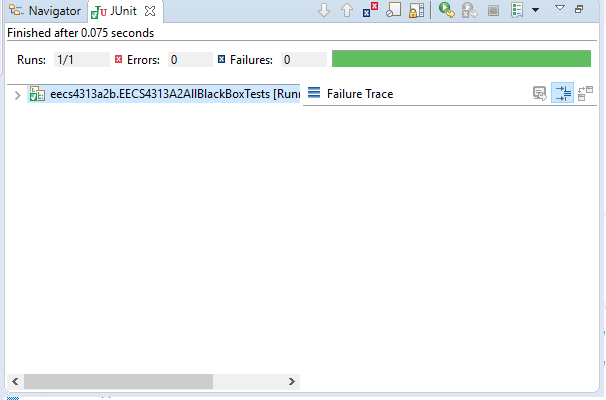
\includegraphics[width=.99\textwidth]{images/wbt/ect/bbt_ect.png}
\end{center}
\caption{Test run result for the minuteString functionn}
\label{fig:bbt_ect_pass}
\end{figure}

\begin{figure}[!htb]
\begin{center}
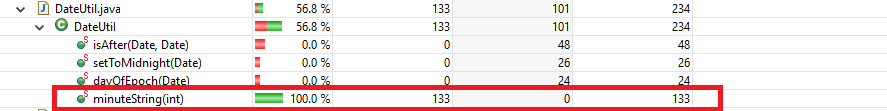
\includegraphics[width=.90\textwidth]{images/wbt/ect/statement_coverage.png}
\end{center}
\caption{Statement Coverage View for the minuteString function}
\label{fig:wbt_ect_code}
\end{figure}

\item \textbf{Additional cases:} Since hours are implemented by dividing integer by 60, the negative integers can produce negative hours . Also, negative hours produced emptystring according to the implementation.However, minutes are computed by taking the reminder of the division ( mins\%60) this will produce a positive number since reminder cannot be negative. Therefore, only two cases we can check in this whitebox testing procedure.They are :
\newpage
 \begin{itemize}
\item Mins/60 $<$ 0 and Mins\%60 $>$ 1 - To test negative hours with more than 1 minut [ Class 10]
 \begin{itemize}
 \item Range of hours: (0,$-\infty$)
 \item Range of minutes: [1]
\end{itemize}
\item Mins/60 $<$ 0 and Mins\%60 = 1 -  To test negative with 1 minute [Class 11]
 \begin{itemize}
 \item Range of hours: (0,$-\infty$)
 \item Range of minutes: (0,59]
\end{itemize}
This covers the two invalid cases possible for the test based on the implementation of the method. since we can only convert negative integers in terms of minutes according to the implementation of the method.This is shown in Figure 3.However these two cases produced a bug because the method is producing negative results instead of positive results since we cannot have negative reminder. this causes the bug. The test cases fail for the two cases are shown in figure 4.


 \end{itemize}



\begin{figure}[!htb]
\begin{center}
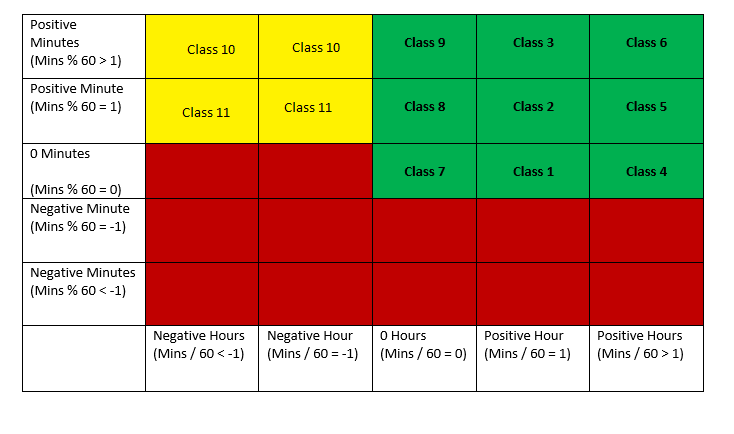
\includegraphics[width=.99\textwidth]{images/wbt/ect/wbtmatrix.png}
\end{center}
\caption{Possible invalid cases for the minuteString function}
\label{fig:wbt_ect_cfg}
\end{figure}
Red coloured boxes in Figure 3 are representing impossible cases since negative integers can be only converted to minutes according to the implementation.Yellow colored boxes show the addtional tests cases that we test in the whitebox and the green boxes are valid outputs that we checked in blackbox test cases.

\begin{figure}[!htb]
\begin{center}
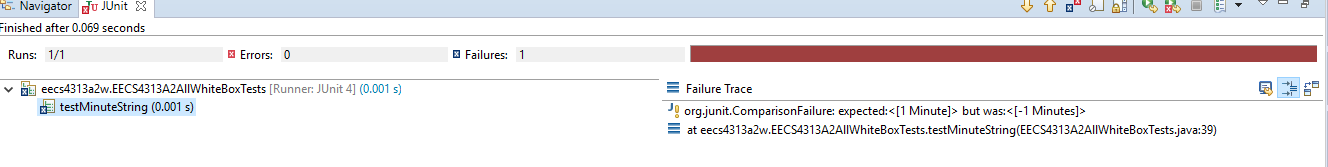
\includegraphics[width=.99\textwidth]{images/wbt/ect/bug.png}
\end{center}
\caption{Additional test cases fail due to a bug in the minuteString function}
\label{fig:wbt_ect_bug}
\end{figure}
\newpage
\newpage

\begin{figure}[!htb]
\begin{center}
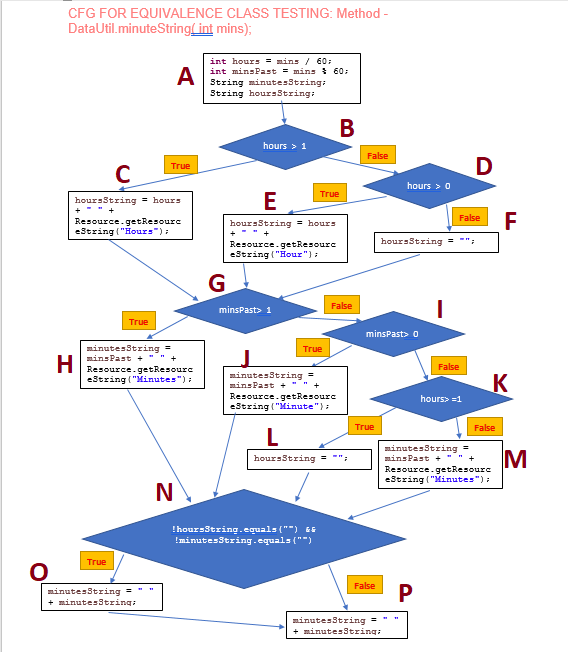
\includegraphics[width=.99\textwidth]{images/wbt/ect/cfg.png}
\end{center}
\caption{Control Flow Graph for the minuteString function}
\label{fig:wbt_ect_cfg}
\end{figure}

%%%%Bug Report%%%%%%%%%%%%%%%%%%%



\subsection{Bug Report}

\begin{itemize}
\item \textbf{Bug Report Title}: DateUtil.minuteString Method does not output the correct result for negative integers
\item \textbf{Reported by}: Kirusanth Thiruchelvam
\item \textbf{Date reported}: March 3, 2018
\item \textbf{Program (or component) name}: net.sf.borg.common.DateUtil.minuteString()
\item \textbf{Configuration(s)}:
\begin{itemize}
\item Operating System: Windows 10 Pro 
\item Version: 10.0.1.16299 Build 16299
\item System Manufacturer: SAMSUNG ELECTRONICS CO., LTD.
\item System Model: QX310/QX410/QX510/SF310/SF410/SF510
\item BIOS: AMIBIOS Version 03MX.M005.20101011.SCY 
\item Processor: Intel(R) Core(TM) i5 CPU   M 460   @ 2.53 GHZ (4CPUs), ~ 2.5GHz
\item Memory: 8192 MB RAM
\item Display Device: Intel(R) HD Graphics (Core i5)
\item BORG Calendar Version: 1.8.3
\item Java Version: 1.8.0\_161
\end{itemize}
\item \textbf{Report type}: Coding Error
\item \textbf{Reproducibility}: 100\%
\item \textbf{Severity}: Low
\item \textbf{Problem summary}: When inputing a negative integer as an argument for the minuteString method in DataUtil class. It produces the number in negative which is not correct since the reminder of the negative integer cannot be ne negaitive.
\item \textbf{Problem description}:\newline
\underline{Steps to Reproduce}
\begin{enumerate}
\item Load the source code of Borg Calender in Java
 \item Create a new junit test case
 \item call the net.sf.borg.common.DateUtil.minuteString() in the class with -70 as an argument
\end {enumerate}
 \underline{ Results}
\item Expected Results: After inputing the -70, it should gives 10 as the output since hour produce empty string and only minutes produce the results.The expected result is to see positive 10 but it gives -10 since (-70) mod 60 is 10 minutes.
\item Real Results: The actual result produce the bug since it shows -10 as the outputs.
\item \textbf{New or old bug}: New
\end{itemize}



\end{itemize}


\end{document}
